\documentclass[border=4pt]{standalone}
\usepackage{tikz}
\usetikzlibrary{arrows.meta,positioning,calc,fit,backgrounds,patterns,shapes.geometric}
\usepackage{amsmath,amssymb}
\usepackage{mathptmx}
\definecolor{lost}{HTML}{C2362D}
\definecolor{kept}{HTML}{17875A}
\definecolor{evid}{HTML}{3056D3}
\definecolor{ink}{HTML}{1D1D1F}
\definecolor{muted}{HTML}{6E6E73}
\tikzset{
  box/.style={draw=ink!70, rounded corners=2pt, align=center, fill=white, inner sep=4pt, font=\footnotesize},
  arr/.style={-{Stealth[length=2mm]}, draw=ink!70, line width=0.6pt},
  grp/.style={draw=muted!60, dashed, rounded corners=4pt, inner sep=7pt},
  lossbox/.style={draw=lost!80, fill=lost!6, text=lost!85!black, rounded corners=2pt, align=left, font=\footnotesize, inner sep=4pt},
  fixbox/.style={draw=kept!80, fill=kept!7, text=kept!65!black, rounded corners=2pt, align=left, font=\footnotesize, inner sep=4pt},
  dec/.style={diamond, aspect=2.2, draw=ink!70, fill=evid!6, align=center, font=\footnotesize, inner sep=1.5pt},
  lbl/.style={font=\footnotesize\bfseries, text=ink},
}

\begin{document}
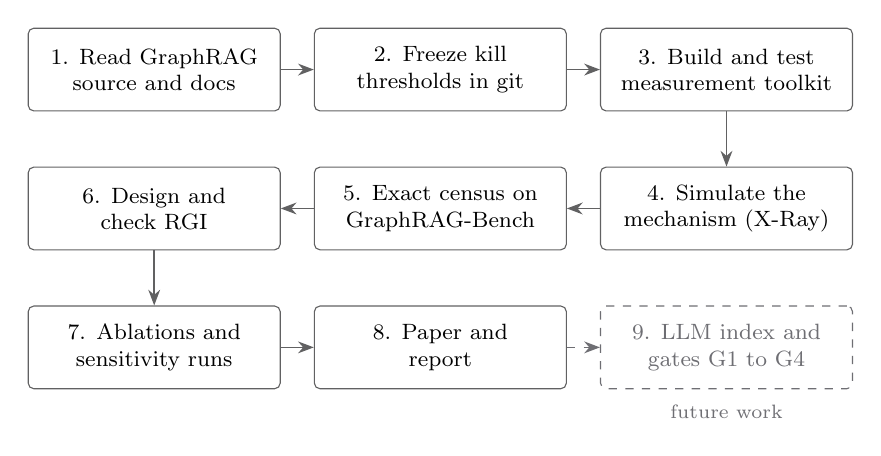
\begin{tikzpicture}[node distance=0.42cm]
\tikzset{st/.style={box, minimum width=3.2cm, minimum height=1.05cm}}
\node[st] (s1) {1. Read GraphRAG\\source and docs};
\node[st, right=of s1] (s2) {2. Freeze kill\\thresholds in git};
\node[st, right=of s2] (s3) {3. Build and test\\measurement toolkit};
\node[st, below=0.7cm of s3] (s4) {4. Simulate the\\mechanism (X-Ray)};
\node[st, left=of s4] (s5) {5. Exact census on\\GraphRAG-Bench};
\node[st, left=of s5] (s6) {6. Design and\\check RGI};
\node[st, below=0.7cm of s6] (s7) {7. Ablations and\\sensitivity runs};
\node[st, right=of s7] (s8) {8. Paper and\\report};
\node[st, right=of s8, draw=muted, text=muted, dashed] (s9) {9. LLM index and\\gates G1 to G4};
\foreach \a/\b in {s1/s2,s2/s3,s3/s4,s4/s5,s5/s6,s6/s7,s7/s8} \draw[arr] (\a) -- (\b);
\draw[arr, dashed, draw=muted] (s8) -- (s9);
\node[font=\scriptsize, text=muted, below=0.08cm of s9] {future work};
\end{tikzpicture}
\end{document}
